\documentclass[a4paper,12pt]{article}

%temporary includes
\usepackage{textcomp} %for arrows in comments

% Remove colours from refs%
\usepackage[hidelinks]{hyperref}

%includes
\usepackage{color}
\usepackage{cite}

% magyar nyelv
\usepackage[magyar]{babel}
\usepackage[utf8]{inputenc}

\usepackage{fixltx2e}
\usepackage{hyperref}

% for set notation
\usepackage{mathbbol}

% for matrices
\usepackage{amsmath}
\usepackage{blkarray}

% for images
\usepackage{graphicx}
\usepackage{float}
\graphicspath{ {img/} }

\DeclareUnicodeCharacter{00A0}{ }
%\DeclareUnicodeCharacter{00A0}{~} % not using no-break space

% sizes
\usepackage{geometry}
\geometry{
    left=25mm,
    right=25mm,
    top=25mm,
    bottom=25mm,
}
% sorköz
\linespread{1.5}

% For tables
\usepackage{array}
\usepackage{calc}

% Equation description
\usepackage{enumitem}

% Adding dots after section numbers
\usepackage{titlesec}
\titlelabel{\thetitle.\quad}


\pdfinfo{%
  /Title    (Bakteriális patogén és ember közötti molekuláris hálózatok vizsgálata)
  /Author   (Horváth Balázs)
  /Creator  ()
  /Producer ()
  /Subject  (MSc Szakdolgozat)
  /Keywords ()
}

%Title page 
%TODO: add more information, logo and stuff as requested
\title{Bakteriális patogén es ember közötti molekuláris hálózatok vizsgálata}
\author{Horváth Balázs}
\date{2015}

\begin{document}
\maketitle
\pagebreak

\section{Tartalomjegyzék}
\pagebreak

\section{Rövidítésjegyzék}
\pagebreak

\section{Bevezetés}
	\subsection{A bél mikrobióta fontosságának ismertetése}
	\subsection{A szakirodalomban publikált gazda patogén hálózatok} 
	\subsection{A Humán-Salmonella kapcsolat ismertetése és hatása az 	autofágiára}
	\subsection{Ökológiai hálózatok elemzésére használt topológiai mérőszámok}
	 
	 \paragraph{Miért van szükség topológiai mérőszámokra?} \mbox{}\\ %linebreak after paragraph title
	 A konzervrációs biológia az élettudományok azon ága mely a Föld biodiverzitásának megőrzésével foglalkozik. Mivel az összes faj védelme nem megoldható, ezért szükségessé vált olyan fajok kiválogatása melyek kiemelt figyelmet igényelnek konzervációs biológiai szempontból.\cite{new_zeland} Az 1990-es évek előtt a védelemre való kiválasztás fő szempontja a faj ritkasága volt.  A fajok ilyen alapú szelekciója nem veszi figyelembe hogy például az adott taxon kulcsszerepet játszik-e az ökoszisztéma funkciók ellátásában. \cite{jordan_comparison}
	 
	 \paragraph{Kulcsfajok} \mbox{}\\ %linebreak after paragraph title
	 1966-ban Robert Paine megalkotta a kulcsfaj koncepciót(\textit{keystone species}). Megfigyelte hogy ha kiesik a Kaliforniai sziklás tengerparti közösségből a \textit{Piaster ochraceus} csúcsragadozó tengeri csillag akkor az egész közösség fajösszetétele összeomlik. A mai legelfogadottabb kulcsfaj definíció szerint ezek olyan fajok, melyek ökológiai hatása aránytalanul nagy az abundanciájukhoz képest. A fogalommal kapcsolatban azonban további kérdések merülnek fel: Milyen hatás számít nagynak? Pontosan mekkora biomassza hányad után mondható az adott faj ereje aránytalannak? \cite{new_zeland} Ez utóbbi kérdések megválaszolásához szükség van olyan mérőszámokra, melyek segítségével kvantitatívvé tehető egy adott faj ökológiai fontossága. Másrészt így lehetővé válik a fajkiválasztás során a szubjektivitás csökkentése is. Az ilyen mérőszámok használatával objektív fontossági sorrendet lehet felállítani az adott élőhelyen előforduló taxonok között. \cite{jordan_comparison} 
	 
	 \paragraph{Rangsorolásra használt topológiai mérőszámok az ökológiában} \mbox{}\\
	 Ma már a kulcsfajok kiválasztása részben ökológiai interakciós hálózatok elemzése alapján történik. A használt hálók kizárólag biotikus-biotikus (faj-faj) kapcsolatokat tartalmaznak. Erre azért van szükség, mert például minden élőlény összekötésben áll a detritusszal és ez eltorzítaná az analízis eredményét. Sőt ilyen esetben a detritusz maga is struktúrális kulcsfajnak számítana. Egy adott fajnak az ökológiai interakciós hálóban betöltött szerepét pozicionális fontossági mérőszámokkal, vagy más néven centralitási indexekkel lehet jellemezni. A konzervációs biológiában sokfajta ilyen mérőszámot használnak, melyeknek közös tulajdonsága, hogy mindegyik valamilyen egyedi tulajdonságra fekteti a hangsúlyt és az alapján rangsorolja a hálózatban szereplő fajokat. Ilyen eltérés lehet két index között például, az hogy az egyik egy adott pont lokális kapcsolati mintázatára, míg a másik az egész hálózatra vonatkozó hatását számszerűsíti. Adott hálóra különböző mérőszámok eltérő fajsorrendeket adnak, de a hasonló tulajdonságok figyelembevételén alapuló mérőszámok között felállíthatók konszenzus fák. \cite{jordan_comparison} \textcolor{red}{ !TODO: esetleg lehetne még kicsit írni arról, hogy sok ökológiai mérőszám igazábol szociológiából jött \textrightarrow  Wasserman, S., Faust, K., 1994. Social Network Analysis. Cambridge University Press,
	 Cambridge. }
	 
	 \paragraph{Főbb topológiai mérőszámok}
	 
	 \paragraph{Normalised degree - D} \mbox{}\\Az adott ponttal kapcsolódó pontok száma elosztva a hálózat összes pontjának számával. \cite{top_indexes}
	 
	 \paragraph{Closeness centrality - CC vagy C } \mbox{}\\ A pontok száma elosztva az adott pontból eredő azt minden más ponttal összekötő legrövidebb topológiai távolságok összegével. \cite{top_indexes} Ez a mérőszám megmutatja, hogy egy adott pontnak mekkora az átlagos távolsága a hálózat összes többi pontjától. Az index kicsi szám olyan pontokra melyek rövid legrövidebb útvonalakon vannak a többi ponttal összekötve. Az ilyen pontok valószínűleg könnyebben elérnek más pontokat vagy nagyobb hatást tudnak gyakorolni más pontokra. Adott $i$ pont átlagos legrövidebb távolságát a többi ponttól a következőképpen lehet kiszámolni: \cite{newman_networks}
	 
	 	\begin{equation}
			\ell_i= \frac{1}{n-1} \sum_{j} d_{ij} \qquad \mathrm{vagy,} \qquad \ell_i= \frac{1}{n} \sum_{j (\neq i)} d_{ij}
	 	\end{equation}
	 	 \noindent{Ahol}:
	 	 \begin{itemize}[label=]
	 	 	\item $\ell_i$ : Az $i$ pont átlagos legrövidebb távolsága a hálózat többi pontjától.
			\item $d_{ij}$ : Az az i pontot a j ponttal összekötő legrövidebb útvonal (geodézikus útvonal) pontjainak száma.
			\item $n$: A hálózat pontjainak száma.
	 	 \end{itemize}
	 
	 A két számítás között stratégiai különbség van. A baloldali egyenlet azt feltételezi, hogy adott pontnak önmagára mért hatása nem releváns a hálózat működésének szempontjából. Azonban még erre az esetre is jellemző, hogy mivel definíció szerint a $d_{ii}$ távolság 0, ezért az összeget ez az érték nem növeli csupán az osztót. \cite{newman_networks}  \\
	 Az $\ell_i$ érték önmagában még nem centralitási index, mert kis számokat ad a magas központiságú pontokra. A megkapjuk a \textit{Closeness Centrality}-t az $\ell_i$ inverzét kell vennünk: \cite{newman_networks}
	 
	 	\begin{equation}
			C = \frac{1}{\ell_i}
	 	\end{equation}
	 
	 \paragraph{Betweenness centrality - BC} \mbox{}\\ 
	 A vizsgálni kívánt ponton áthaladó a hálózat többi pontpárját összekötő legrövidebb utak összege elosztva a hálózat többi pontpárját összekötő összes legrövidebb út összegével.  \cite{top_indexes} 	 Ez a mérőszám azt mutatja meg, hogy egy adott pont milyen arányban szerepel a többi pont között futó útvonalakban. A \textit{betweenness centrality} vagy röviden  \textit{betweenness} olyan hálózatok jó jellemzője, melyekben valamilyen természetű ``áramlás" folyik a pontok között. Ha feltételezzük, hogy egy ilyen hálózat minden kapcsolata között az áramlás során ugyanannyi kicserélődés történik egy egységnyi idő alatt és a kicserélődés a legrövidebb útvonalakon folyik, akkor az összes geodézikus útvonalon is azonos rátával történik az áramlás. Ez azt jelenti, hogy egy adott ponton átmenő áramlás mennyisége arányos azzal, hogy a hálózat legrövidebb útvonalainak milyen arányában szerepel. \cite{newman_networks}
	 
  	 \paragraph{Information Centrality - IC} \textcolor{red}{ !TODO}
	 
	 \paragraph{Topological importance - TI\textsuperscript{n}}  \mbox{}\\
	 Ez egy teljesen topológiai alapú mérőszám mely összegzi az egy adott pontból kiinduló összes lehetséges \textit{n} lépéshosszúságú útvonal hatását. A hálózat összes direkt kapcsolatára kiszámítható azok topológiai erőssége:
	 
	 \begin{equation}
		d_{X,Y} = \frac{1}{x}
	 \end{equation}
	 
 	 \noindent{Ahol}:
 	 \begin{itemize}[label=]
		 \item $d_{X,Y}$ : Az Y pont hatása X pontra.
		 \item $x$ : Az X pont első szomszédainak száma.
 	 \end{itemize}
	 
	 Az így kiszámolt közvetlen kapcsolatok hatását egy mátrixban lehet ábrázolni, melynek indexelése a populációdinamika konvencióit követi: \textit{d}\textsubscript{\textit{ij}} jelenti a \textit{j} pontnak az \textit{i} pontra gyakorolt hatását. Adott direkt kapcsolat hatásának nagysága a kapcsolat irányától is függ, tehát \textit{d}\textsubscript{\textit{ij}} nem feltétlenül ugyanakkora mint \textit{d}\textsubscript{\textit{ji}}. Egy \textit{n} lépés hosszú útvonal erejét az ezt alkotó direkt kapcsolatok hatásának szorzataként értelmezzük:
	 
	 \begin{equation}
		d^n_{p_{XY}} =\prod_{i=1}^{n-1} d^1_{i, i+1} 
	 \end{equation}
	 
	 
	 \noindent{Ahol}:
	 \begin{itemize}[label=]
		 \item $p_{XY}$: Útvonal amire igaz hogy $p \in$ \{$X$ és $Y$ közötti $n$ lépés hosszúságú útvonalak\}
		 \item $d^n_{p_{XY}}$: Az $X$ és $Y$ pontok közötti $n$ lépés hosszú $p$ útvonal ereje.
		 \item $d^1_{n, n+1}$: Az útvonal $i$ és $i+1$-ik pontja közötti direkt kapcsolat erőssége
	 \end{itemize}
	 
	  \noindent{Ez alapján egy $Y$ pont hatása $X$-ra $n$ lépés távolságban:}
	 
	 \begin{equation}
		 d^n_{XY} = \sum d^{n}_{p_{XY}}
	 \end{equation}
	 \noindent{Ahol}:
	 \begin{itemize}[label=]
		\item $p_{XY}$: Útvonal amire igaz hogy $p \in$ \{$X$ és $Y$ közötti $n$ lépés hosszúságú útvonalak\}
		\item $d^n_{XY}$: Az összes $Y$ pontból eredő és $X$-ben végződő $n$ hosszúságú útvonalak erejének összege. 
	 \end{itemize}	 
	 
	 Mivel a direkt kapcsolatok ereje függ a kapcsolat irányától, így a TI tükrözi a kapcsolat asszimmetrikusságát is. Egy adott pontra TI\textsuperscript{n} a következő képen számítható ki:
	 
	 \begin{equation}
		\textrm{TI}^n_A=\sum d^n_{j,A}
	 \end{equation}
	 
	 \noindent{Ahol}:
	 \begin{itemize}[label=]
		 \item  $\textrm{TI}^n_A$: $A$ pont $n$ lépésre számított topológiai fontossága.
		 \item  $d_{j,A}$: $A$ és $j$ pont közötti $n$ hosszúságú útvonalak ereje. 
	 \end{itemize}
	 
	A TI$^n$-t a hálózat összes pontjára ki lehet számítani és ez alapján sorrendet lehet felállítani a nódusok között.
	 
 	 \begin{figure}[H]
 		 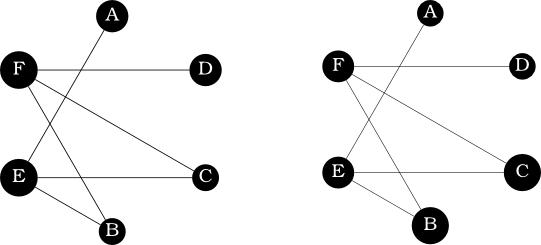
\includegraphics[scale=1]{img/graphs.png}
 		 \centering
 		 \caption{$d$ \textit{(bal)} és TI\textsuperscript{2} \textit{(jobb)} szemléltetése ugyanazon a példagráfon }
 		 A pontok átmérője arányos az adott nódusra kiszámolt $d$ (direkt vagy közvetlen topológiai kölcsönhatás) és TI$^2$ (topológiai fontosság két lépésre) értékekkel. \cite{ti} alapján módosítva.
 		 \label{fig:peldagraph}
 	 \end{figure}
 	 
 	 Az \ref{fig:peldagraph}. ábrán látható példagráfra rendre felírhatóak a közvetlen  kölcsönhatások ($d$) és a két lépésnyire közvetített indirekt kölcsönhatások ($d^2$) értékeit tartalmazó mátrixok:
	
	% Példamátrixok %
	\[
	\begin{blockarray}{ccccccc}
	&A & B & C & D & E & F \\
	\begin{block}{c [cccccc]}
	A &0 & 0 & 0 & 0 & \frac{1}{3} & 0 \\[6pt] 
	B & 0 & 0 & 0 & 0 & \frac{1}{3} & \frac{1}{3}\\[6pt] 
	C & 0 & 0 & 0 & 0 & \frac{1}{3} & \frac{1}{3}\\[6pt] 
	D & 0 & 0 & 0 & 0 & 0 & \frac{1}{3}\\[6pt] 
	E & 1 & \frac{1}{2} & \frac{1}{2} & 0 & 0 & 0\\ [6pt] 
	F & 0 & \frac{1}{2} & \frac{1}{2} & 1 & 0 & 0\\ [6pt]
	\end{block}
	\multicolumn{7}{c}{\indent $d$ értékek} \\ [6pt]
	\end{blockarray},\quad
	\begin{blockarray}{ccccccc}
	&A & B & C & D & E & F \\ 
	\begin{block}{c [cccccc]}
	A & \frac{1}{3} & \frac{1}{6} & \frac{1}{6} & 0 & 0 & 0 \\[6pt] 
	B & \frac{1}{3} & \frac{1}{3} & \frac{1}{3} & \frac{1}{3} & 0 & 0\\ [6pt] 
	C & \frac{1}{3} & \frac{1}{3} & \frac{1}{3} & \frac{1}{3} & 0 & 0\\[6pt] 
	D & 0 & \frac{1}{6} & \frac{1}{6} & \frac{1}{3} & 0 & 0\\[6pt] 
	E & 0 & 0 & 0 & 0 & \frac{2}{3} & \frac{1}{3}\\ [6pt] 
	F & 0 & 0 & 0 & 0 & \frac{1}{3} & \frac{2}{3}\\ [6pt]
	\end{block}
	\multicolumn{7}{c}{\indent $d^2$ értékek} \\[6pt]
	\end{blockarray}
	\]
	
	Az ábrázolt mátrixok elrendezése követi a populációdinamikai konvenciókat, tehát például $d_{BF}=\frac{1}{2}$ azt jelenti, hogy $F$ pont a $B$-re $\frac{1}{2}$ erővel hat. Mindkét mátrixra érvényes az, hogy az adott oszlop értékeinek összege egy. Ez a tulajdonság a $d$ érték definíciójából fakad. $d$ azt mutatja meg, hogy adott pont a cél pont kapcsolatainak hányad részét adja. Ezáltal minden pont egy egységnyi hatást kap ami eloszlik a vele kapcsolatban álló pontok között. \cite{ti} Ezt a hatást jól szemlélteti az \ref{fig:peldagraph}. ábra jobb oldali része amin látható, hogy $B$, $C$, $D$ és $A$ pontok kimenő hatása kisebb, mivel célpontjaik sok hatást fogadnak. \\
	\indent Ugyancsak mindkét mátrixra jellemző, hogy a sorok összege azt mutatja meg, hogy egy adott pont mennyire erős kölcsönható, tehát mekkora TI$^n$ értéke. Például $B$ pont két lépés távolságban összesen $\frac{4}{3}$ erővel hat, ez alapján erősebb kölcsönhatónak mondható mint az $A$ pont a maga $\frac{2}{3}$ értékű összesített kimenő két lépés hosszú hatásaival. \cite{ti} \\
	\indent Az \ref{fig:peldagraph}. ábrán az is jól megfigyelhető, hogy $C$ pont a gyengébb közvetlen kölcsönhatók közé tartozik. Ugyanakkor mivel a $C$-ből eredő két lépéses útvonalak erős elsődleges kölcsönhatókon keresztül érik el végpontjaikat, ezáltal két lépés távolság viszonylatában már $C$ is az erős kölcsönhatók közé tartozik. \\
	\indent Az $n > 1$ lépésszámú $d^n$ értékeket tartalmazó mátrixokban már egy adott pont indirekt hatása önmagára is kiterjedhet. Páros számú lépések esetén viszont mindenképpen felírhatók olyan útvonalak melyeken a pont eléri önmagát, \cite{ti} vagyis $d^n_{X,X} \neq 0$ ha n $\in$ \{ $2k :  k \in \mathbb{Z}$ \}. Az \ref{fig:peldagraph}. ábrán látszik, hogy például az $F$ pont két lépés távolságban a következű útvonalakon hat önmagára: $F \rightarrow B \rightarrow F$, $F \rightarrow C \rightarrow F$ és  $F \rightarrow D \rightarrow F$.
	
 	 \paragraph{Weighted Topological Importance - WI\textsuperscript{n}} \textcolor{red}{ !TODO}

\section{Források és módszertan}

	\subsection{Adatbázisok}
		\subsubsection{SLK3 Layer 0 összeállítása és ebből a Rho útvonal extrakciója}
		\subsubsection{Arn Core}
		\subsubsection{Salmonet}
		\subsubsection{Predictions}

	\subsection{Az adatbázisok egyesítése}
		\subsubsection{Algoritmusok leírása}
		\subsubsection{Módszerek és technológiák leírása}

	\subsection{Az egyesített hálózat elemzésének módszere}
		\subsubsection{Topológiai mérőszámok jellemzői}
		\subsubsection{Algoritmusok, alkalmazott technológiák}

\section{Eredmények (A hálózat elemzése)}
	\subsection{Főbb statisztikák}
	\subsection{Kapott topológiai adatok és jelentésük}
	
\section{Diszkusszió}
\section{Összefoglalás}
\section{Summary}
\section{Hivatkozások jegyzéke}
\section{Köszönetnyilvánítás}
\section{Nyilatkozat}


\bibliography{msc_szakdolgozat}{}
\bibliographystyle{apalike}

\end{document}

